\documentclass[12pt,a4paper,french] {article}

\pagestyle{empty}

\usepackage{../../Style}

\renewcommand{\baselinestretch}{1.25}

\begin{document}
 
\titre{Activité - Fonctions}

\compo[0.4] {
$ABCD$ est un rectangle de dimension 4 et 6 cm. E est un point mobile de $[BC]$, et $EBFG$ est un carré. On étudie l'aire de la zone hachurée, qui dépend de la position de $E$ sur $[BC]$. On note $x=BE$ pour $x \in [0;4]$.}
{\center{\includegraphics[scale=0.7]{Activité.png}}}

\begin{enumerate}

\item Justifier que $x \in [0;4]$.
\item Déterminer une expression de l'aire $f(x)$ de la zone hachurée.
\item Vérifier que $f(x)=2x^2-10x+24$
\item Compléter la table de valeurs suivantes à l'aide de la calculatrice:

\begin{center}
\begin{tabularx}{\linewidth}{ 
  | >{\centering\arraybackslash}c 
  | >{\centering\arraybackslash}X
  | >{\centering\arraybackslash}X
  | >{\centering\arraybackslash}X
  | >{\centering\arraybackslash}X
  | >{\centering\arraybackslash}X
  | >{\centering\arraybackslash}X
  | >{\centering\arraybackslash}X
  | >{\centering\arraybackslash}X
  | >{\centering\arraybackslash}X | } \hline
$x$ & 0 & 0.5 & 1 & 1.5 & 2 & 2.5 & 3 & 3.5 & 4 \\ \hline
$f(x)$ &  & & & & & & & & \rule[-7pt]{0pt}{40pt} \\ \hline
\end{tabularx}
\end{center}

\compo[0.35] {
\item Tracer l'allure de la courbe de cette fonction et vérifier que l'on obtient:

\item Résoudre graphiquement l'inéquation $f(x) > 16$
\item Trouver graphiquement les extremums de $f$.
}
{\begin{center}
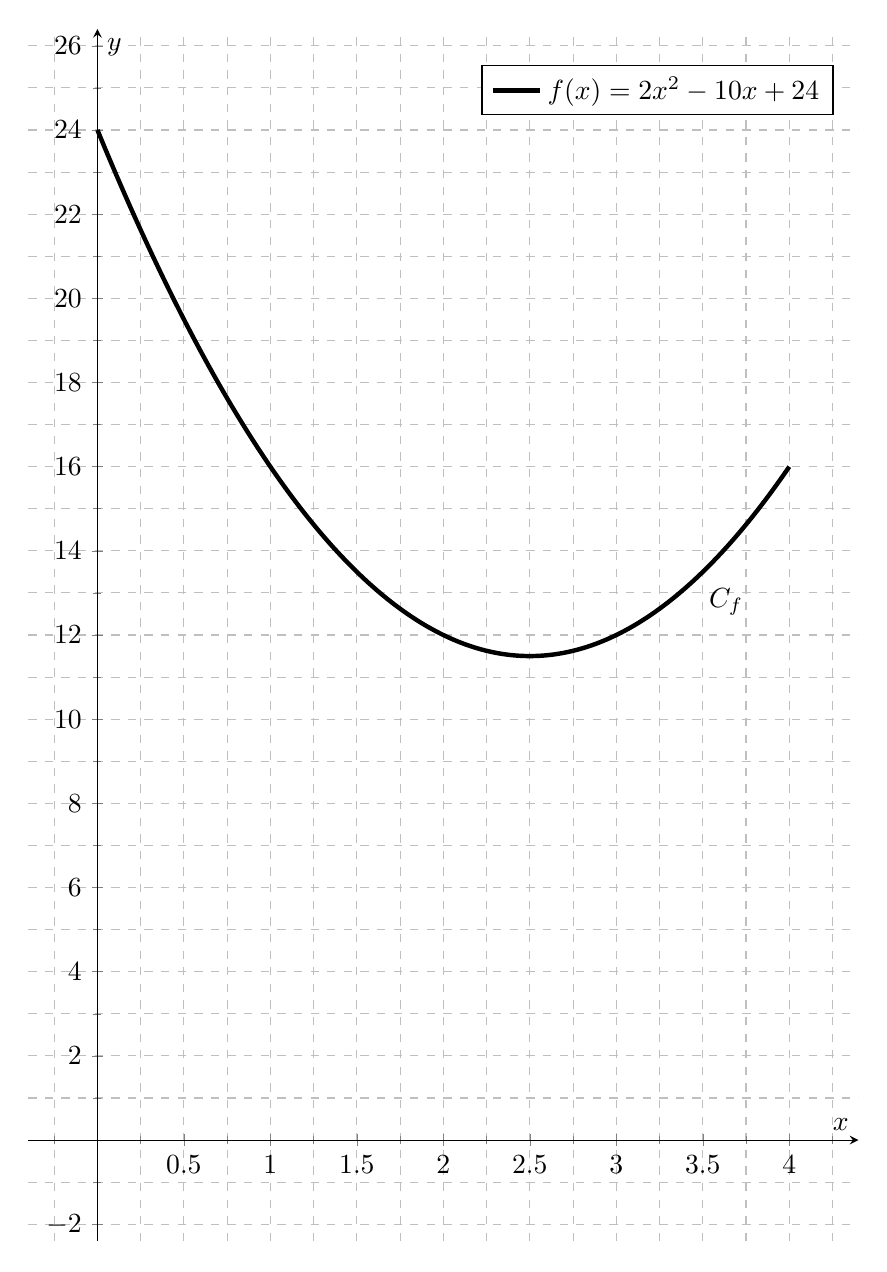
\begin{tikzpicture}[scale=1]
\begin{axis}[
axis x line=bottom,
axis y line = left,
axis lines=middle,
width=\linewidth,
height=1.4*\linewidth,
xmin=0, xmax=4,
ymin=0, ymax=24,
enlargelimits={0.1},
xlabel={$x$},
ylabel={$y$},
minor x tick num=1,
minor y tick num=1,
%ytick distance=1,
grid=both,
grid style=dashed,
%axis equal,
legend pos=north east,
]
\addplot[samples=101,smooth,ultra thick,domain=(0:4),mark=none]{2*x^2-10*x+24} node [pos=0.85,below right] {$\mathscr C_f$};
\addlegendentry{$f(x)=2x^2-10x+24$};
%\pgfplotsinvokeforeach{-1.5,-1,...,2.5}{ \node[circle, minimum size=2pt,fill,color=red,inner sep=2pt] at (axis cs:#1,#1*#1-#1) {};};
\end{axis}
\end{tikzpicture}
\end{center}}

\end{enumerate}

\end{document}
